\documentclass[11pt,a4paper]{article}
\usepackage[left=2cm,text={17cm,25cm},top=2.5cm]{geometry}
\usepackage[T1]{fontenc}
\usepackage[english]{babel}
\usepackage[utf8]{inputenc}
\usepackage{url}
\usepackage{graphicx}
\usepackage{pdfpages}
\usepackage[colorinlistoftodos,prependcaption,textsize=tiny]{todonotes}

\graphicspath{ {figs/} }

\begin{document}

\begin{center}
	\LARGE{Soft Computing}\\
	\Large{Job Performance Evaluation Using Back-propagation Network}
	\vspace{0.5cm}

    \begin{centering}
    \small{
        Bc. Petr Stehlík <xstehl14@stud.fit.vutbr.cz>
        }
    \end{centering}

	\vspace{0.2cm}

\end{center}

\section{Introduction}
Every user of a supercomputer needs to know whether their submitted job finished successfully and performed well. So far these tedious tasks are usually performed manually using only the output of their program and over-simplified metrics such as job runtime and total utilized resources.

The aim of this project is to create a back-propagation neural network which can classify whether a job ran well or if it is in some way suspicious of unwanted behaviours such as poor performance or execution failure.

The network itself is supplied with fine-granular metric data acquired via Examon framework\cite{examon} which was run on Galileo supercomputer located in CINECA, Bologna, Italy. Where all job and metric data were gathered.

The structure of this document is as follows: in section \ref{sec:theory} the theoretical background needed for this project is presented together with the description of Examon framework. In the following section \ref{sec:data} the data supplied to the network are described as well as the final format of the data. Afterwards, in section \ref{sec:implementation} the implementation of the network and its structure are laid out and in the last two sections \ref{sec:res} and \ref{sec:sum} the achieved results, summary and further work are discussed.

\section{Theoretical Background}
\label{sec:theory}

\subsection{Backpropagation Network}
Backpropagation networks are multi-layer feed-forward networks with supervised learning. There is no interconnection between neurons in the same layer but layers are fully connected to the next neighbouring layer in order to be able to do forward and backward propagation of values.

\subsubsection{Forward-propagation}
Each neuron in all layers but input layer disposes of a weight for each input initialized to a random value in range $<0,1>$, linear base function and sigmoidal activation function.

When forward propagating an input vector the vector is laid out onto the input neurons and the vector is recalculated using following formulas for the next layer until the input vector is propagated to the output layer which outputs the response of the whole network itself.

The base function is shown in equation \ref{eq:base}:

\begin{equation}
    f(\vec{x}) =\sum_{i = 0}^{n} w_i x_i
    \label{eq:base}
%    f(u) = \frac{1}{1 + e^{-\lambda u}}
\end{equation}

where $ \vec{x} $ is the input vector, $ w $ are weights for each input of given neuron and $ n $ is the length of the neuron input vector and bias (term used as in \cite{deeplearning}\cite{elements}) value resulting in $ n = |x| + 1$.

The sigmoidal activation function is presented in equation \ref{eq:act} where $ \lambda $ is a constant set to $ \lambda = 1 $ and in further equations left out because of this fact.

\begin{equation}
    g(u) = \frac{1}{1 + e^{-\lambda u}}
    \label{eq:act}
\end{equation}

The output of a neuron is then given by using the equations \ref{eq:base} and \ref{eq:act}:

\begin{equation}
    y = g( f( \vec{x} ) )
    \label{eq:output}
\end{equation}


\subsubsection{Back-propagation}
Back-propagation is used only when one trains the network and is one of the base methods for training feed-forward networks. The method is based on adjusting weights depending on the error calculated by equation \ref{eq:err} for an output neuron $ p $ using produced output ($ o $) and desired output ($ d $) values.

\begin{equation}
    E_p = \frac{1}{2} \sum_{j = 1}^{m} (d_{pj} - o_{pj})^2
    \label{eq:err}
\end{equation}

The change of weights is calculated using equation \ref{eq:delta} where $ \nabla E_p $ is the derived error gradient and $ \mu $ the learning rate.

\begin{equation}
    \Delta \vec{w_p} = -\mu \nabla E_p
    \label{eq:delta}
\end{equation}

To calculate one particular change of weight we use formula \ref{eq:neuron-delta} where $ L $ is the given layer of the network, $ j $ is the $j$-th neuron in layer $ L $ and $ i $ is the $i$-th input of the neuron $ j $.

\begin{equation}
    \Delta w_{ji}^L = \mu \delta_j^L x_i^L
    \label{eq:neuron-delta}
\end{equation}

For the output layer $ L $ of the network we use formula \ref{eq:output-err}.

\begin{equation}
    \delta_j^L = (d_j - y_j^L) y_j^L(1 - y_j^L)
    \label{eq:output-err}
\end{equation}

For hidden layers of the network, we use the same principle propagating the error backwards from the output layer as shown in equation \ref{eq:prop-err} where $\lambda = 1$ and therefore left out.

\begin{equation}
    \Delta {^l w}_{ji} = \mu {^l\delta}_j {^lx}_i = \mu \sum_{k = 1}^{n_{l+1}} (^{l+1}\delta_k {^{l+1}w}_{kj}) {^ly}_j (1 - ^ly_j){^lx}_i
    \label{eq:prop-err}
\end{equation}

Each repetition of forward and backward propagation of all inputs is called an epoch. Finally, we can choose when to update the weights, in batches after all input vectors were processed or using the stochastic method where weights are updated after processing each input vector.

\subsection{Examon}
\label{sec:examon}
Examon\cite{examon} framework is used for exascale monitoring of supercomputing facilities. It is built on top of MQTT protocol\cite{locke2010mqtt} which allows measured metrics to be sent to a central broker where received data are processed and stored in KairosDB\cite{KAIROS} database utilizing Cassandra\cite{CASSANDRA} cluster.

\begin{figure}[ht]
    \centering
    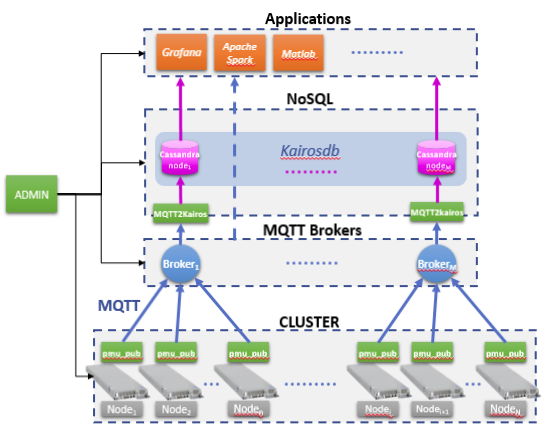
\includegraphics[width=0.45\linewidth]{examon-architecture}
    \caption{Examon framework architecture}
    \label{arch}
\end{figure}

KairosDB is used for storing metric data in time-series format whereas Cassandra, serving as a backend for KairosDB is also used for storing job-related data. More on data semantics is described~in~\ref{sec:data}.



\section{Data}
\label{sec:data}

As previously stated in \ref{sec:examon} data are gather via Examon framework and stored in Cassandra database. We can split the data into two categories. Job data and metric data.

The job data come from 


\section{Implementation}
In this section, we describe the implementation phase of the project. The project was implemented using Python 2.7.13. External library SciPy\cite{scipy} was used for linear data interpolation.

\label{sec:implementation}

\subsection{Data Acquisition}
\label{sec:data-filter}
First, job data were queried and filtered according to several rules:
\begin{itemize}
    \item job run time must be between 10 and 60 minutes
    \item job must occupy the whole node (multiplies of 16 cores)
    \item job must be run in 15-day period
\end{itemize}

This resulted in 32 jobs which gave enough diversity for correct classification. All datapoints were aggregated by 30 seconds using averaging aggregator available in KairosDB.

The rule of minimum 10 minutes is because of any shorter job is usually a development, not production version of a program and in current HPC facilities such program is very cheap to run and therefore no deep performance analysis is needed. The same goes for jobs smaller than one node (16 cores).

Jobs longer than one hour are not suited for training the network because of too large input vectors exceeding the scope of this project and the loss of information in further data processing.

\subsection{Data Labelling}
In order to correctly label all chosen jobs and their metrics a simple graphical user interface was made. The GUI is based on previous work done during the PRACE Summer of HPC called Examon Web which is an extension of Examon framework visualizing specific views of all collected data.

Visualization is done in timeseries fashion using Dygraphs library. This helps to better understand the correlations between all metrics and in time combined.

The GUI is shown in figure \ref{fig:ex-labeler} where you can see a check box for each metric and at the bottom a checkbox for the whole job. The metric checkbox labels the accompanying metric of suspicious behaviour and job one of suspicious behaviour of the job as a whole.

\begin{figure}[ht]
    \centering
    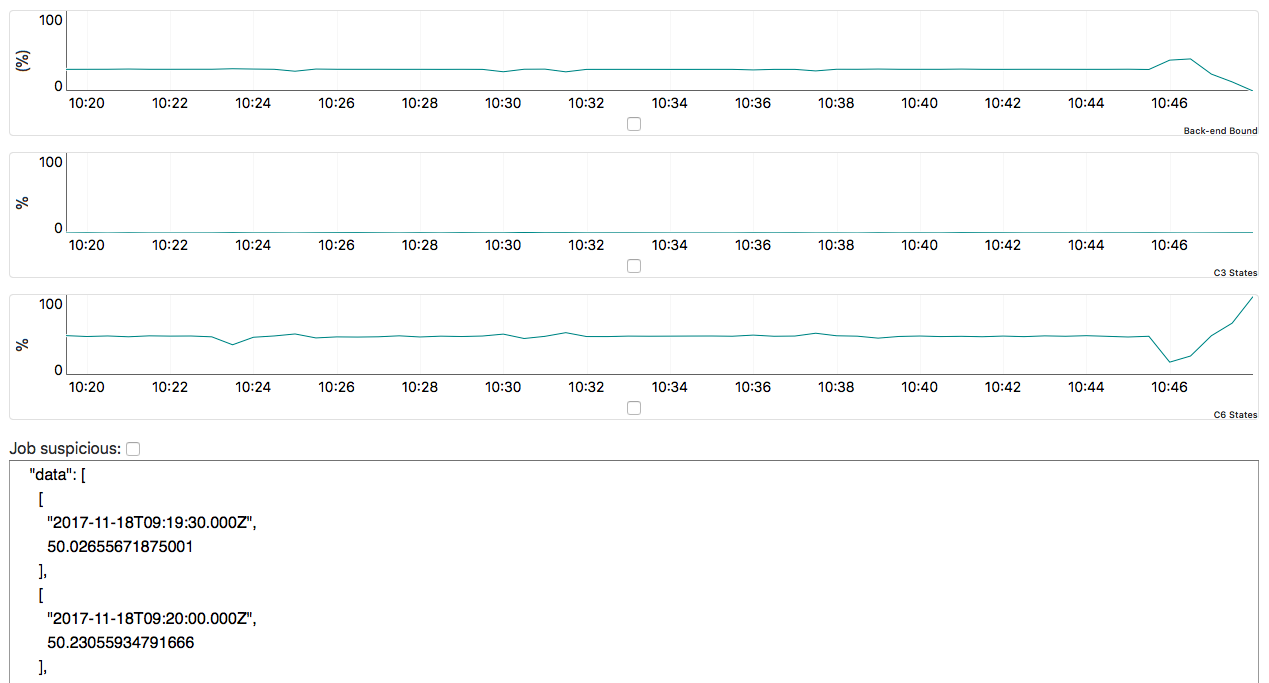
\includegraphics[width=0.75\linewidth]{examon-labeler}
    \caption{Part of Examon Web based data labelling tool}
    \label{fig:ex-labeler}
\end{figure}

\subsection{Data Processing}

After labelling the job all metric data with labels are generated and can be worked on further. All metric vectors were interpolated to 80 values which provides good performance/detail compromise. Larger input vectors resulted in extremely longer runs and smaller input vectors resulted in poor outputs of the network.

\subsection{Metric Networks}

To achieve best results/speed combination a backpropagation neural network was created for each metric. This gives us the total of twelve networks completely independent of each other which means the training process can be fully parallelized.

All metric networks were configured the same way to achieve uniform results. The input layer disposes of 80 neurons with hidden layers of 4 and then 3 neurons and one output neuron.

This configuration was chosen based on trial and error experiments.

\subsection{Job Network}
Once all metric networks compute their output we have a vector of 12 values which serves as an input to the job classification network.

The network is created with 12 input neurons, one hidden layer of 4 neurons and one output neuron.

All networks output a single value. Metric networks because of further processing in the job network and the job network because of clearer values.


\section{Achieved Results}
\label{sec:res}

The sum error was calculated using equation \ref{eq:err}. Each metric had its sum error as presented in table \ref{tab:errors}. As one can see the sum error varies through the dataset but sum errors below $1.0$ can be considered as acceptable. The largest error comes from core's load and CPU utilization since these two metrics are very similar.

\begin{table}[ht]
    \parbox{.48\linewidth}{
        \centering
        \begin{tabular}{lll}
        Name                    & Epochs & Sum Error \\
        core's load             & 49999  & 5.81947   \\
        C6 states               & 1506   & 0.07591   \\
        C3 states               & 4      & 0.09447   \\
        instructions per second & 49999  & 3.18977   \\
        system utilization      & 17988  & 0.09695   \\
        CPU utilization         & 49999  & 7.65817   \\
        IO utilization          & 49999  & 0.94946   \\
        memory utilization      & 49999  & 0.82774   \\
        L1 and L2 bounds        & 49999  & 0.52690   \\
        L3 bounds               & 49999  & 0.77589   \\
        front-end bounds        & 49999  & 2.72293   \\
        back-end bounds         & 49999  & 4.63103   \\
        job classifier          & 49999  & 0.73037
        \end{tabular}
        \caption{Overview of sum errors for all networks}
        \label{tab:errors}
    }
    \hfill
    \parbox{.48\linewidth}{
        \centering
        \begin{tabular}{lll}
        Job \# & Expected & Result \\
        1   & 0 & 0.04   \\
        2   & 0 & 0.05   \\
        3   & 0 & 0.58   \\
        4   & 1 & 1.0    \\
        5   & 1 & 0.96
        \end{tabular}
        \caption{Sum error for job evaluation dataset}
        \label{tab:joberr}
    }

\end{table}

Even with these sum errors the job classifier labelled the evaluation dataset correctly with minor errors as seen in table \ref{tab:joberr}

\section{Summary}
\label{sec:sum}

As a proof of concept for classifying jobs on HPC cluster, it was verified that such classification can be made using a set of backpropagation networks. With rather a small dataset to train and evaluate the networks the error rate wasn't minimal and can be further reduced using a larger labelled dataset and users' feedback.

The dataset itself cannot be randomly generated because of too complex dependencies between all metrics. Having randomly generated data we even couldn't determine whether such artificial job would be really suspicious or not.

Using the intermediate input from metric networks it can be used for intelligent dashboards in Examon Web where only suspicious metrics can be shown in combination with several fixed ones.

This work is the base for my master thesis and will be further expanded to provide complex insights on users' jobs suggesting the possible cause of the suspicious behaviour.

\section{Program Manual}

The Python code can be run using command \texttt{python jobclassifier} from the root folder of the project. The program makes available following arguments:
\begin{itemize}
       % \setlength\itemsep{0em}
    \item \texttt{-h, -{}-help} show help
    \item \texttt{-{}-train} train the networks using \texttt{data.json} dataset
    \item \texttt{-{}-dir CONFIG\_DIR} where to store configurations for trained networks
    \item \texttt{-{}-max-epochs EPOCHS} train the network using \texttt{data.json} dataset (default: 10 000)
    \item \texttt{-{}-eval CONFIG\_EVAL} maximum number of epochs
\end{itemize}

An example command for training the networks: \texttt{python jobclassifier -{}-train -{}-dir example} and example command for evaluating the dataset using networks trained from previous example: \texttt{python jobclassifier -{}-eval example}.


\subsection*{Acknowledgements}
This work was done using the Examon framework created by F. Beneventi, A. Bartolini, A. Borghesi and collective at UNIBO, Italy. Examon Web was created by P. Stehlík during the PRACE Summer of HPC stay at CINECA, Bologna, Italy. Data used in this project were collected using the CINECA infrastructure and Galileo supercomputer and anonymized before any use in this project.

\bibliography{doc}{}
\bibliographystyle{abbrv}

\end{document}
